\documentclass[10pt,twoside,a4paper]{amsart}
\usepackage[ascii]{inputenc}
\usepackage[LGR,T1]{fontenc}
\usepackage[english]{babel}
\usepackage{amsmath}
\usepackage{amssymb,amsfonts,textcomp}
\usepackage{array}
\usepackage{hhline}
% \usepackage{hyperref}
\usepackage{graphicx}

\author{Leif R. Uppstr\"om}
\address{L. Uppstr\"om, L\"onnv\"agen 29, 513 35 Fristad, Sweden}
\email{luppstrom@live.se}
\author{Daniel Uppstr\"om}
\title{Prime Numbers as a Function of a Geometric Progression}

\begin{document}

\maketitle

\begin{abstract}
In mathematical literature it is asked for a computable function or efficient algorithm to find all, or at least a large subset, of the prime numbers. This paper shows that all primes can be characerised by their reciprocal period length $L$ and its figure value $R$. These parameters are given for each prime after inversion to an infinitely repeated period and are used to group all primes into disjoint sets that arise as a function of a geometric progression. This theory suggests new ways to enumerate and find large primes.
\end{abstract}

\section{Introduction}

The purpose of this paper is to obtain a general formula for all prime numbers and explain their arising pattern. The work is based on the specific property of prime numbers, that each of them can be inverted to give an infinitely repeated period of integers characterised by two parameters, its length $L$, equal to the period number of digits, and its figure value $R$ without the introductory zeroes \cite{Ore}. The reciprocal length $L$ of the small prime numbers ${\leq}$5 will be considered separately as will the few primes consisting of the repeated digit 1 only \cite{Beiler}.

Primes with the same L-value can be defined to be members of families $A_{L} = \{p_{1},p_{2},p_{3},...\}_{L}$; $L = 1,2,3...$, that are disjoint and together contain all prime numbers, $\cup A_{L}=\mathbb{P}$, with every family containing at least one prime. The maximum number of primes in a family is limited to a relatively small and foreseeable number. When searching for family members it is essential to know if the periodic length $L$ is a prime or a composite number. This is however automatically determined in advance if the search is performed in numerical order of $L = 1,2,3...$. The prime numbers obtained from families generated in numerical order of $L = 1,2,3...$ will be called original primes (op), when they appear for the first time. This is always the case when $L$ itself is a prime. If $L$ is a composite number it will be shown that some smaller and earlier in the series found original prime(s) are repeated in the resulting $R$-value, which therefore demands a correction to get the proper family $A_{L}$. Those recurrent primes are said to be complementary (cp) and are excluded.

An important equation is $p-1 = LU$ ; $p{\textgreater}5$, where $L$ is the reciprocal period length of $1/p$ and $U$ is an integer. This equation is used to show that products of prime numbers with the same $L$ also get the same $L$, and furthermore to demonstrate that the amount of primes with equal $L$ are limited in number. 

The families $A_{L}$ can be linked to the geometric series $(10^{L} - 1)/9$, called repunit numbers \cite{Beiler}, the series of the infinitely repeated digit 1, thus 1, 11, 111, 1111\ldots etc. which abbreviated can be written $(1)_{L}$. Every family consisting of primes with the same period length $L$ has an original and complete solution within this infinite progression. With this knowledge it is possible to create an algorithm to find all primes. They will then appear in the order of their reciprocal period length, not in order of the prime values themselves. Note, however, that the relation to the natural sequence of prime numbers is elucidated in part \ref{sect:pattern}.

\section{Inversion of Prime Numbers}

When the number 1 is divided by a prime $p>5$, there is only $p-1$ possible remainders in each step of division. As soon as a remainder repeats itself a period is formed and the calculation starts from the very beginning again. Thus, no inverted prime number $p > 5$ can have a repeated period length $L$ that is longer than $p-1$ digits. But $L$ could be shorter, a digital fraction of $p-1$. This results in the equation, where $U$ is an integer,

\begin{equation}
\label{eq:plu}
p-1 = LU.
\end{equation}

The reciprocal period of any $1/p$ , $(p \neq  2;5)$, is as follows
\begin{equation}
\label{eq:b}
1/p=0.\underbrace{a_{1}a_{2}a_{3}...a_{N}\overbrace{r_{1}r_{2}r_{3}...r_{M}}^{R}}_{\text{period with length L}}a_{1}a_{2}a_{3}...a_{N}r_{1}r_{2}r_{3}...r_{M}a_{1}...
\end{equation}

where $a_{1}$\ldots $a_{N}$ are zeroes (for primes {\textgreater}7), $r_{1}\neq 0$; $r_{M} \neq 0$; $R = r_{1}...r_{M}$, a sequence of digits ending on 1,3,7 or 9. Example: $1/271 = 0,0036900369\ldots$ with $L = 5$ and $R = 369$.


\section{The Connection Between Inverted Prime Numbers and a Geometric Progression}
\label{sect:cbipn}
Let the infinite fraction $1/p = P$. The equation \ref{eq:b} is multiplied with $10^{L} = (100...0)$, where $L$ is the length of the reciprocal period.
\begin{equation}
\label{eq:c}
10^{L}P = 10^{L}(.a_{1}a_{2}a_{3}...a_{N}r_{1}r_{2}r_{3}...r_{M}a_{1}a_{2}a_{3}...a_{N}r_{1}r_{2}r_{3}...r_{M}...)
\end{equation}
$P$ is subtracted from both sides to give $(999\ldots{}9)P = a_{1}a_{2}a_{3}\ldots{}a_{N}r_{1}r_{2}r_{3}\ldots{}r_{M}$, followed by division with 9 to give $(111\ldots{}1)P = R/9$.\\
Define the periodic number value $T = R/9$ and then, because $P = 1/p$, the final result is
\begin{equation}
\label{eq:d}
(111...1) = pT.
\end{equation}
This equation shows, that all prime numbers with period length $L$, are factors of the corresponding repunit number,  
\begin{equation}
\label{eq:primeprod}
(1)_{L} = p_{1}\cdot p_{2}\cdot \ldots \cdot p_{N}\cdot C,
\end{equation}
where $C$ is the remaining, yet unknown, factor.\\
But there is one difficulty to be observed. If a number in the geometric progression (of repunit numbers) is a single prime itself, solely consisting of a row of the digit 1, then $L$ must also be a prime, but it is still not possible to see the difference between those numbers being prime or composite. That is because every inversion $1/(1)_{L}$ gives $T = 1$. This is shown by comparison of some examples:
\\
\begin{itemize}
\item[] $L=2$, $(1)_{2}$, $1/11=0.090909\ldots$, $T=R/9=1$ and 11 is a prime number,\\
\item[] $L=5$, $(1)_{5}$, $1/11111=0.0000900009\ldots$, $T=R/9=1$ but $11111 = 41\cdot 271$ composite,\\
\item[] $L=19$, $(1)_{19}$, $1/1111111111111111111 = 0000000000000000009\ldots$, $T = 1$, a prime.\\
\end{itemize}

Prime numbers in the progression $(10^{L} - 1)/9$ consisting of a row of the digit 1 are very rare; only four numbers {\textgreater}11 are known so far: $(1)_{19}$, $(1)_{23}$, $(1)_{317}$ and $(1)_{1031}$ \cite{Ribenboim}. Next number in that series (if any) must according to Dubner have more than 10 000 digits \cite{Dubner}. Every such prime number makes a single-member family $A_{L}$.\\
\\
Another more important obstacle is, however, that the nature of $L$ in the calculation above, equation \ref{eq:c}, must be considered. $L$ can be either a prime or a composite number and the knowledge is of great significance.

\subsection{The Period Length $L$ is a Prime Number}

If $L$ is a prime, all the eventual factors of $T$ must have the same reciprocal length $L$ as the inverted $p$ to form the product $(10^{L}-1)/9 = pT$. This is shown as follows. Let $p_{1}$ and $p_{2}$ have the same $L$ and apply a set of equation \ref{eq:plu},
\begin{equation*}
p_{1} = LU_{1} + 1
\end{equation*}
and
\begin{equation*}
p_{2} = LU_{2} + 1
\end{equation*}
which multiplied gives
\begin{equation*}
p_{1}p_{2}-1 = L(LU_{1}U_{2} + U_{1} + U_{2})
\end{equation*}
where $L$ is the same as in each of the equations above, only the new $U$-value is increased and dependent on the L-value. Further multiplication with primes of the same reciprocal length $L$ gives

\begin{equation}
\label{eq:prodlu}
\prod_{n}p_{n}-1 = L\tilde{U}
\end{equation}

and the product of all multiplied factors must have the same $L$. This is verified by the inversion of the final product $1/(1)_{L} = 0.00\ldots{}09$ with the same $L$. Thus, when $L$ is prime,
\begin{equation}
\label{eq:prodLprime}
(10^{L}-1)/9 = (1)_{L}=\prod_{n}p_{n},
\end{equation}
giving $C=1$ in equation \ref{eq:primeprod}.\\
\\
The following relations also hold, for $L$ being prime:
\begin{equation*}
T_{1} = p_{2}p_{3}p_{4}\ldots{}p_{N}
\end{equation*}
\begin{equation*}
T_{2} = p_{1}p_{3}p_{4}\ldots{}p_{N}
\end{equation*}
\begin{equation*}
T_{3} = p_{1}p_{2}p_{4}\ldots{}p_{N}
\end{equation*}
\begin{center}
$\ldots$
\end{center}
\begin{equation*}
T_{N} = p_{1}p_{2}p_{3}\ldots{}p_{N-1}
\end{equation*}
\begin{equation}
\label{eq:e}
(10^{L}-1)/9 = (1)_{L} = p_{1}T_{1}= p_{2}T_{2} = p_{3}T_{3} =\ldots{}=P_{N}T_{N},
\end{equation}
where all primes belong to the same family
\begin{equation}
\label{eq:f}
A_{L} = \{p_{1},p_{2},p_{3},\ldots{},p_{N}\}.
\end{equation}

When $L$ is prime all the factors appear for the first time in the progression $(10^{L} - 1)/9$, $L = 1,2,3\ldots$ and are original primes.

\subsection{The Period Length $L$ is a Composite Number}
\label{subsect:tplcn}
If the reciprocal period length $L$ is a composite number $L_{c}$, a number of primes with shorter period length values $l_{n}$ ,where $1<l_{n}<L_{c}$ and $L_{c}/l_{n}$ is an integer, will interfere. An $l_{n}$ can sometimes correspond to more than one prime. This is illustrated by a typical example.\\

Let $L_{c} = 15$ which has the two divisors $l_{1} = 3$ and $l_{2} = 5$.\\

Prime numbers 3 and 37 which have a period length $l = 3$ that exactly divides $L_{c} = 15$ can thus be repeated. Prime numbers 41 and 271 have a period length $l = 5$ dividing $L_{c}$ and are repeated likewise. This is not the case if smaller primes have a periodic length of, e.g. $L = 6$, or any other $L$-value that does not divide $L_{c}$ giving integers. Thus
\begin{equation*}
(10^{15}-1)/9 = (1)_{15} = \underset{L_{c}=15}{31} \cdot \underset{L_{c}=15}{2906161} \cdot \underset{l=3}{3} \cdot \underset{l=3}{37} \cdot \underset{l=5}{41} \cdot \underset{l=5}{271}.
\end{equation*}
\begin{equation*}
\text{The family } A_{15} = \{31, 2906161\}.
\end{equation*}
This can also be shown in general terms:\\
Let $p_{1}-1 = LU_{1}$ and $p_{2}-1 = l_{2}U_{2}$ where $l_{2} = L/m$ ; $L$ is composite and m is an integer.\\
Then $p_{1} = LU_{1}+1$ and $p_{2} = LU_{2}/m + 1$ and
\begin{equation}
\label{eq:gencomp}
p_{1}p_{2} - 1 = (LU_{1} + 1)(LU_{2}/m) = L(LU_{1}U_{2}/m + U_{1} + U_{2}/m)
\end{equation}
The product is calculated the same way as was equation \ref{eq:prodlu}; the $L$-value for the product remains constant, however, the $U$-value is different when taken care of the particular primes with shorter lengths. This shows why the equation \ref{eq:d} cannot distinguish between $L$ being prime or composite and why prime numbers with shorter $L$-values must be eliminated to find the proper $A_{L}$ family. \\
If prime numbers $p_{n}$ are inverted and their period lengths are the same composite $L_{c}$ and smaller prime numbers $q_{n}$ with shorter lengths $l_{n}$ where $1<l_{n}<L_{c}$ and $L_{c}/l_{n} = m$ are present either of the following results is obtained:
\begin{itemize}
\item[] $1/p_{1} = p_{2}\cdot p_{3}\cdot p_{4}\cdot ...\cdot p_{N}\cdot q_{1}\cdot q_{2}\cdot q_{3}\cdot ...\cdot q_{M} = T_{1}$
\item[] $1/p_{2} = p_{1}\cdot p_{3}\cdot p_{4}\cdot ...\cdot p_{N}\cdot q_{1}\cdot q_{2}\cdot q_{3}\cdot ...\cdot q_{M} = T_{2}$
\item[] $\ldots$
\item[] $1/p_{N} = p_{1}\cdot p_{2}\cdot p_{3}\cdot ...\cdot p_{N-1}\cdot q_{1}\cdot q_{2}\cdot q_{3}\cdot ...\cdot q_{M} = T_{N}$
\end{itemize}
Let $q_{1}\cdot q_{2}\cdot ...\cdot q_{M} = C$ to correct for primes of shorter lengths and obtain the product of the members of the requested family
\begin{equation}
\label{eq:prodALc}
\prod{A_{L_{c}}} = p_{N}T_{N}/C = p_{1}\cdot p_{2}\cdot p_{3}\cdot \ldots \cdot p_{N}
\end{equation}
A table of some prime numbers is generated to show the difference between the periodic lengths when $L$ is prime or composite and also to illustrate how original primes change to complementary. 

\begin{table}[h!]
\begin{tabular}{c c c c}
primes $\in A_{L}$ & & factors of $C_{L}$ & $\prod A_{L}\cdot C_{L}$ \\
Original primes op & $L$ & complementary primes cp & \\
\hline
11 & 2 & 1 & $(1)_{2}$\\
3; 37 & 3 & 1 & $(1)_{3}$\\
101 & 4 & 11 & $(1)_{4}$\\
41;271 & 5 & 1 & $(1)_{5}$\\
7;13 & 6 & 11;3;37 & $(1)_{6}$\\
239;4649 & 7 & 1 & $(1)_{7}$\\
73;137 & 8 & 11;101 & $(1)_{8}$\\
333667 & 9 & $3^2$;37 & $(1)_{9}$\\
9091 & 10 & 11;41;271 & $(1)_{10}$\\
21649;513239 & 11 & 1 & $(1)_{11}$\\
9901 & 12 & 3;7;11;13;37;101 & $(1)_{12}$\\
53;79;265371653 & 13 & 1 & $(1)_{13}$\\
909091 & 14 & 11;239;4649 & $(1)_{14}$\\
31;2906161 & 15 & 3;37;41;271 & $(1)_{15}$\\
17;5882353 & 16 & 11;101;73;137 & $(1)_{16}$\\
2071723;5363222357 & 17 & 1 & $(1)_{17}$\\
19;52579 & 18 & $3^{2}$;7;11;13;37;333667 & $(1)_{18}$\\
$(1)_{19}$ & 19 & 1 & $(1)_{19}$\\
3541;27961 & 20 & 11;41;101;271;9091 & $(1)_{20}$\\ 
\end{tabular}
\caption{Prime numbers generated according to the geometrical series $(10^{L}-1)/9$; $L=2\ldots20$.}
\label{primetable}
\end{table}

As an example the prime number 11 is an original prime for $L = 2$ and a complementary prime from $L = 4$ and then for every second $L$ and so on. Sometimes, as can be seen for $L = 9$, a small factor is repeated, necessary to make the value a complete row of the digit 1, in this case $(1)_{9}$, which then can be found in the multiples of complementary primes e.g. for $L = 18$ and so on. It might be necessary to control the primality by dividing with the smallest complementary factors again as e.g. for $L=9$ etc. and $L=22$, depending on how the determination of the primes is performed.

\subsection{Elementary applications}

Using for example the new pattern seen in table \ref{primetable} it is possible to obtain series of larger primes by multiplying known $L$-primes, thus being in control of the complementary primes and the reciprocal length of the searched prime numbers. Some simple examples might illustrate.\\
\\
Find the original prime numbers of: \emph{a)} $(1)_{14}$, \emph{b)} $(1)_{44}$, \emph{c)} $(1)_{64}$.\\
\\
Every prime number or product of prime numbers ($p\neq 2;5$) with the same reciprocal length $L$ divides some shortest number consisting of a row of $L$ digits of unit 1. If two $L$-values, both prime, are multiplied, the result is a new $L$ with one or more original prime numbers, (as the initial prime numbers have no complementary primes, the $A_{L}$ is rather easily calculated, see a) below). If instead a product of $L$-values give a new $L$, that is divisible in more than one way, one has to observe that the complementary primes should be eliminated in accord with the product of equation \ref{eq:prodALc} but not counted twice in general. However, see the remark in the last sentence of 3.2 \cite{Book1}.\\
\\
Answer:
\begin{itemize}
\item[] \emph{a)} Let $L_{1} = 2$ and $L_{2} = 7$, then $L_{1} \cdot L_{2} = 14$. Primes in $A_{2}$ and $A_{7}$ are now complementary. Thus $(1)_{14}/((1)_{2}\cdot (1)_{7}) = 909091 \text{ (prime)} \in A_{14}$
\item[] \emph{b)} $L = 44$ can have factors 2, 4, 11 and 22 and $(1)_{44} = 89 \cdot 1052788969 \cdot 1056689261 \cdot 11^{2} \cdot 23 \cdot 101 \cdot 4093 \cdot 8779 \cdot 21649 \cdot 513239$. The three first numbers are original prime numbers and the rest complementary primes to be omitted, (previous original primes for 2, 4, 11 and 22, which can partly be seen in Table \ref{primetable}. Original primes for $L = 22$ is 23, 4093 and 8779). Then $A_{44} = \text{\{the first three numbers\}}$.
\item[] \emph{c)} $L = 64$ with factors $2^{n}$ is an example of how series of numbers could be built up as long as required. Table \ref{table:2n} is self-instructive.
\end{itemize}

\begin{table}[h!]
\begin{tabular}{l l l l}

$2^{n}$ & $L$ & $(1)_{n}$ & Prime number factors\\
\hline
$2^{1}$ & 2 & $(1)_{2}$ & $\mathbf{11}$\\
$2^{2}$ & 4 & $(1)_{4}$ & $11\cdot \mathbf{101}$\\
$2^{3}$ & 8 & $(1)_{8}$ & $11\cdot 101\cdot \mathbf{73} \cdot \mathbf{137}$\\
$2^{4}$ & 16 & $(1)_{16}$ & $11\cdot 101\cdot 73\cdot 137\cdot \mathbf{17}\cdot \mathbf{5882353}$\\
$2^{5}$ & 32 & $(1)_{32}$ & $(1)_{16}\cdot \mathbf{353}\cdot \mathbf{449}\cdot \mathbf{641}\cdot \mathbf{1409}\cdot \mathbf{69857}$\\
$2^{6}$ & 64 & $(1)_{64}$ & $(1)_{32}\cdot \mathbf{19841}\cdot \mathbf{976193}\cdot \mathbf{6187457} \cdot \mathbf{834427406578561}$\\
$2^{7}$ & 128 & $(1)_{128}$ & $(1)_{64}\cdot \mathbf{1(0)_{63}1}$\\
$2^{8}$ & 256 & $(1)_{256}$ & $(1)_{128}\cdot \mathbf{1(0)_{127}1}$\\
etc. & & & 
\end{tabular}
\caption{Formation of a series of primes with control of known complementary primes. The original primes for each $L$ is marked with extra bold type. To find the original primes for e.g. the reciprocal length $L = 128$ the calculation is $(1)_{128} /(1)_{64} = 1(0)_{63}1$. The number $1(0)_{63}1$, to be resolved, contains all primes with that $L$.}
\label{table:2n}
\end{table}

\section{Inversion of the Minor Prime Numbers ${\leq}$5}

The prime numbers 2 and 5 do not give infinitely repeated periods if inverted, $1/2 = 0.5$, $1/5 = 0.2$ and $L=0$. If, however, 0.2 and 0.5 are looked upon as 0.19999... and 0.49999... respectively, the result will be $L = 1$, $R = 9$ and $T = 1$ as a consequence, which might be applied.

The smallest odd prime 3 is more interesting since it has two possible length values $L = 1$ and $L = 3$. As a fact $1/3 = 0.3333\ldots$ but it is not quite obvious that the period should be $L = 1$ except for the two first digits 3. If multiplied $3\cdot 3 = 9$ and $1/9 = 0.1111\ldots$ the result is $L = 1$, but $1/3^{3}$ gives $1/27 = 0.037037\ldots$ with $L = 3$. As a consequence of equation \ref{eq:e} for prime numbers when $L$ is a prime, $(10^{3}-1)/9 = 111 = 37 \cdot 3$ and the number 3 is an original prime number because $L = 3$; $R = 27$ and $T = R/9 = 3$. The first two digits 3 disappear by the compulsory division of $R$. The smallest primes can thus be integrated in our final formula for all prime numbers.

\section{A Conclusive General Formula for Prime Numbers} 

Every prime number {\textgreater}5 can be inverted resulting in an infinitely repeated period, each with a certain length $L$, which also coincides with $L$ in the geometric progression $(10^{L}-1)/9$; $L = 1,2,3\ldots \infty$. This means that all prime numbers with the same $L$ are enclosed as a product in a corresponding step of the progression, thus forming the defined family $A_{L} = \{p_{1},p_{2},p_{3},...,p_{N}\}$. It is, however, absolutely necessary to know whether $L$ is a prime or a composite number to be able to calculate the prime numbers properly, as has been outlined in the previous sections. This has been put together in a comprehensive formula.\\

All prime numbers are enclosed in the union of the infinite number of disjoint families $A_{L}$
\begin{equation}
\label{eq:allprimes}
\mathbb{P}=\bigcup_{L=1}^{\infty}A_{L}
\end{equation}
and, it has been shown, that for every $L$, the product of the elements $p_{n}$ of $A_{L}$ satisfy
\begin{equation}
\label{eq:AL}
\prod A_{L} = \prod_{n}p_{n}=(1)_{L}/C
\end{equation}
where $(1)_{L} = (10^{L}-1)/9$, $C=1$ if $L$ is prime or, if $L$ is a composite number, $C=q_{1}\cdot{}q_{2}\cdot{}q_{3}\ldots$; the product of complementary primes with lengths\  $l_{i}$ : $1<l_{i}<L$ and $L/l_{i}$ an integer. 

\section{The Pattern of the Prime Numbers}
\label{sect:pattern}
The wish to have a simple prime number function of the natural sequence of numbers \cite{Ribenboim} is both directly and indirectly fulfilled here. However, the prime numbers are by definition presented as product families, which instead are a function of a geometric progression. The formulas above, \ref{eq:allprimes} and \ref{eq:AL}, generates primes in the numerical order of their, through inversion $(1/p)$ found, infinitely repeated periodic length $L$. This method yields theoretically all prime numbers and its usefulness is in principle depending only on an efficient data system.\\

\begin{figure}
\centering
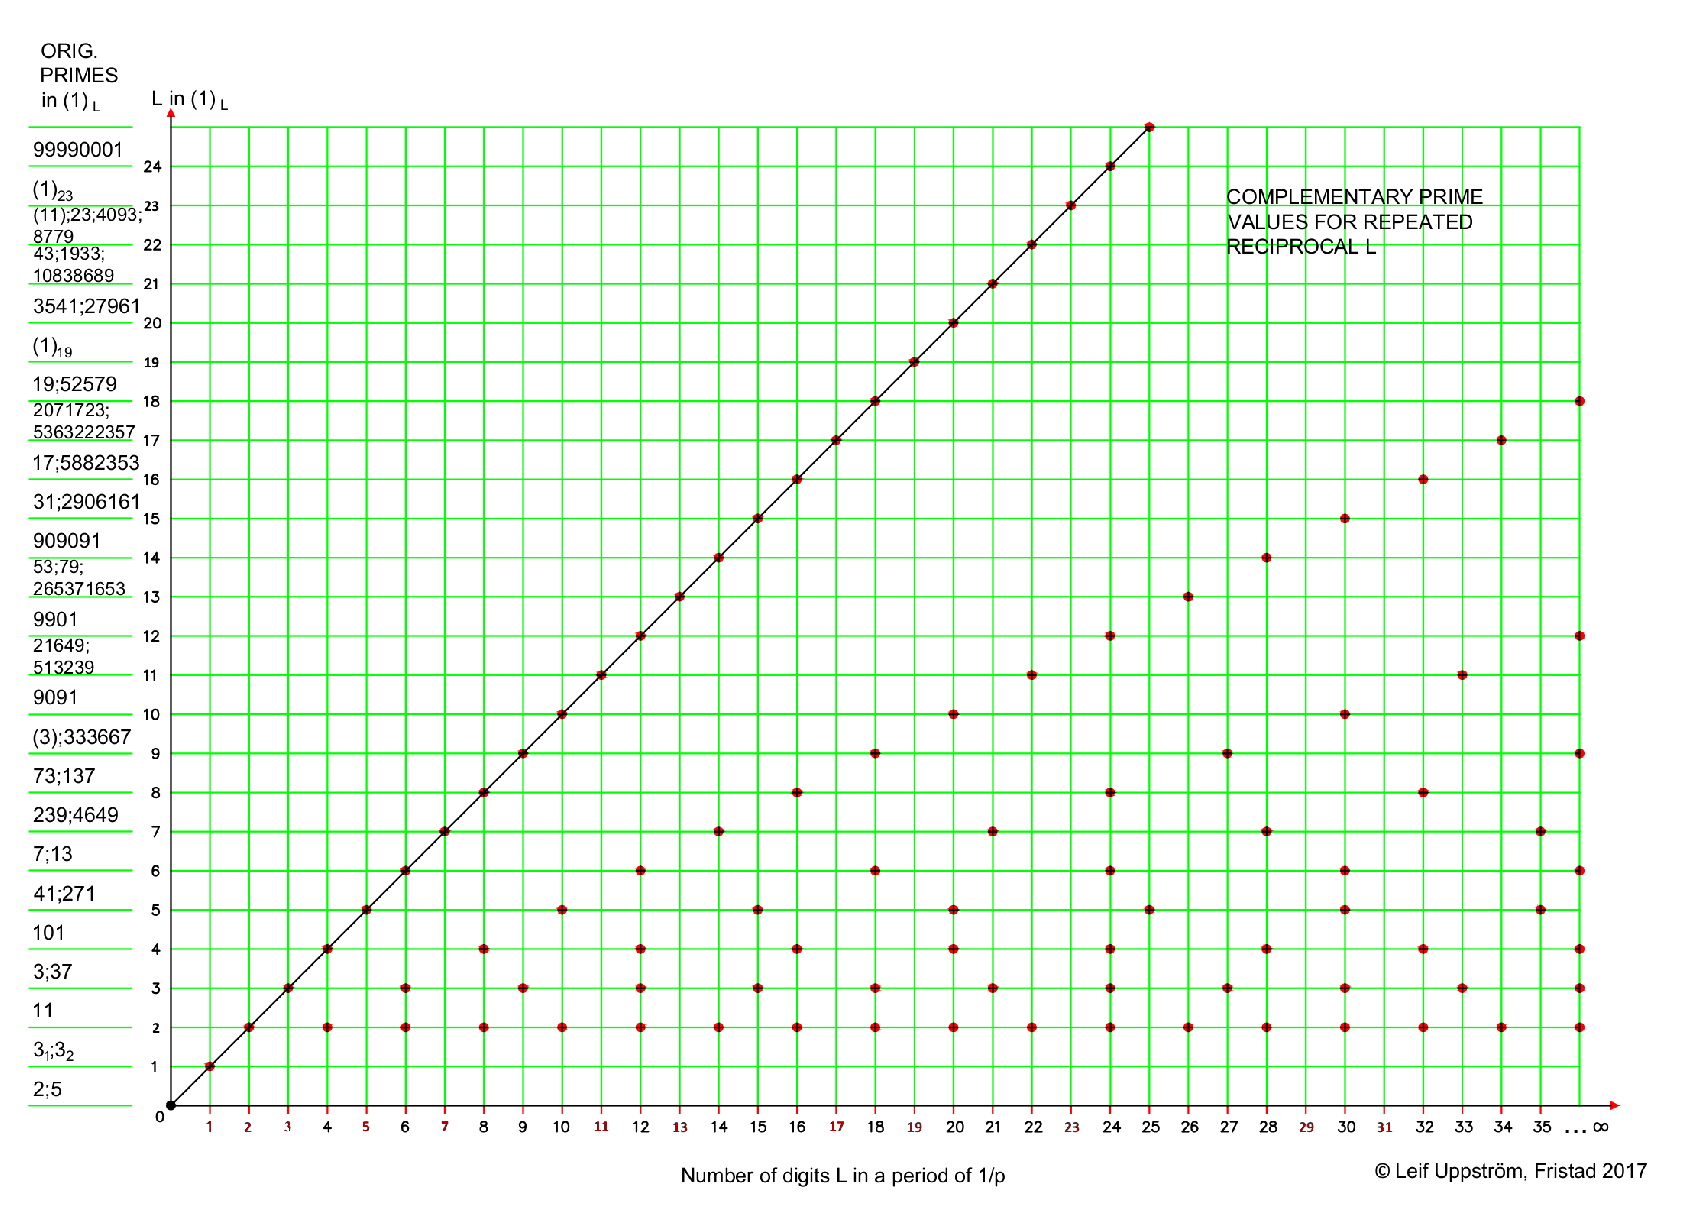
\includegraphics[angle=90,scale=0.7]{diagram.eps}
\caption{This diagram illustrates the established relation between the period length of a prime number and the prime factors in the corresponding term of the series of repunit numbers.}
\label{fig:aa}
\end{figure}

Figure \ref{fig:aa} illustrates the relation between the period length of a prime number and the prime factors in the corresponding term of the (geometrical) series of repunit numbers;\\
1. The diagonal is the line formed by the number $(1)_L$ of repunit digits as a function of the reciprocal length values of the inverted prime number families $A_{L}$; $L = 1,2,3...$. The table along the y-axis contains original prime numbers obtained for each repunit number. On the right hand side of the diagonal all reciprocal lengths are repeatedly marked with dots. By the argument in section \ref{subsect:tplcn} the dots indicate where there are complementary primes for composite $(1)_L$ values.\\
This can be illustrated by an example: The prime number $9091$, in the table at the y-axis, has $L=10$. Move straight to the diagonal and follow the line down to the x-axis. As $10$ is divisible by $5$ and $2$ the complementary primes are found in the table to the left at the position of the dots, ($41$;$271$) and ($11$) respectively. Thus $(1)_{10}=9091\cdot 41\cdot 271\cdot 11$. Complementary numbers are thus relatively easy to find by searching the dividends to $p-1$.\\
2. For products $(1)_L$, where $L$ is a prime, no complementary primes are present. Consequently the lines downwards from the diagonal are free from dots where the L-value on the x-axis is a prime number.\\
This together demonstrates the relationship between the suggested theory and the described linear algorithm.\\
\\
Remark: One has to be aware of the fact that for $(1)_L$, the number $L$ is equal to the number of digits 1 as well as the reciprocal length value. But even if $L$ is prime the number $(1)_L$ is very seldom a single prime itself. See section \ref{sect:cbipn}.\\    
\\
The described procedure of generating prime numbers, theoretically unlimited, is besides the sieve of Eratosthenes perhaps the only complete method. The main difference between these two methods is, that the sieve is probably more time consuming depending on the necessary elimination of the non-primes. On the other hand, the new method presents the primes as families which are a function of the geometric series $(10^{L}-1)/9$, and not a function of the natural sequence of numbers. This means that every prime {\textgreater}5 divides a row of the digit 1 (shortest possible, but also multiples of that row). As all the family products end on the digit 1, the visual pattern of large but limited series of prime numbers must probably deviate from the results obtained by Lemke Oliver and Soundararajan in a recent paper \cite{Soundararajan}.\\
\\
Acknowledgement. The authors are indebted to Peter Al{\aa}sen for data treatment.


\begin{thebibliography}{99}

\bibitem{Ore}Oystein Ore, Number Theory and its History, mc Graw-Hill, 1976, ch 13.
\bibitem{Beiler}Albert H. Beiler, Recreations in the Theory of Numbers, Dover Publ. 2nd ed 1966, ch XI.
\bibitem{Ribenboim}Paulo Ribenboim, The Little Book of Big Primes, Springer Verlag, 1991, p 172-3.
\bibitem{Dubner}H. C. Williams and H. Dubner, Math. Comp. 47 1986, p 703-712.
\bibitem{Book1}Leif R. Uppstr\"om and Peter Al{\aa}sen, Math Enigma Vanished, Sj\"olanda, Fristad, Sweden, 2015, ISBN 978-91-637-9869-6.
\bibitem{Soundararajan}R. J. Lemke Oliver and K. Soundararajan, Unexpected Biases in the Distribution of Consecutive Primes. arXiv:1603.03720v2, 15 Mar 2016.
\end{thebibliography}
\end{document}
